%%%%%%%%%%%%%%%%%%%%%%%%%%%%%%%%%%%%%%%%%%%%%%%
%%%     Declarations (skip to Begin Document, line 88, for parts you fill in)
%%%%%%%%%%%%%%%%%%%%%%%%%%%%%%%%%%%%%%%%%%%%%%%

%%\documentclass[10pt]{article}
%%\documentclass[10pt]{report}
%%\documentclass[letterpaper]{article}
\documentclass[12pt]{article}
\usepackage{geometry}
%\usepackage{xcolor}
\usepackage[table]{xcolor}
\usepackage{amsmath}
\usepackage[some]{background}
%\usepackage{lipsum}
%\usepackage{natbib}
\usepackage[utf8]{inputenc} % set input encoding to utf8

% V E R S I O N I N G
\usepackage{vhistory}

% U N I T S
%\usepackage[binary-units]{siunitx}
\usepackage[]{siunitx}

% L I N E  N U M B E R S
\usepackage{lineno}
%\linenumbers
 
% C I T A T I O N S
%\usepackage[backend=biber,style=apa]{biblatex}
\usepackage[backend=biber, style=apa, maxcitenames=1]{biblatex} 
%\DeclareLanguageMapping{english}{english-apa}
%\usepackage{apacite}
%\bibliographystyle{apa}

%\usepackage{biblatex} 
\addbibresource{paperpile.bib}
\usepackage{datetime}

%\usepackage{hyperref}

% Tables
\usepackage{float}
\usepackage[utf8]{inputenc}
\usepackage{tabularx}
\usepackage{booktabs}
\usepackage{longtable}

\usepackage{diagbox} %table split headers
\usepackage{longtable}
\usepackage{array}
\usepackage{rotating}
\usepackage{eqparbox}
\usepackage{makecell, caption, booktabs}
\usepackage{tablefootnote}

\usepackage{colortbl}

% Confusion Table
\usepackage{rotating}
\usepackage{xparse}
\usepackage{booktabs, makecell, multirow}
\NewExpandableDocumentCommand\mcc{O{1}m}
    {\multicolumn{#1}{c}{#2}}
\usepackage{siunitx}

% W A T E R M A R K 
% This gets rid of the draft watermark on the title page
\backgroundsetup{contents={}}
%\usepackage[text=DRAFT]{draftwatermark}

% L I N E  S P A C I N G
%\renewcommand{\baselinestretch}{1.5} 

% This does not have the effect I wanted, putting the caption at the bottom.
%\usepackage{caption}
%\captionsetup[table]{position=bottom} 

% Stuff needed to get table to span pages
\usepackage{enumitem}
%\usepackage{array, booktabs, longtable}
\newcolumntype{x}[1]{>{\raggedright}p{#1}}

\usepackage{etoolbox}
\AtBeginEnvironment{longtable}{%
    \setlist[itemize]{nosep,     % <-- new list setup
                      topsep     = 0pt       ,
                      partopsep  = 0pt       ,
                      leftmargin = *         ,
                      label      = $\bullet$ ,
                      before     = \vspace{-\baselineskip},
                      after      = \vspace{-0.5\baselineskip}
                        }
                           }% end of AtBeginEnvironment
% End table span

\definecolor{green}{rgb}{0.1,0.1,0.1}
%\color{green!40!yellow})

\newcommand{\done}{\cellcolor{teal}done}  %{0.9}
\newcommand{\hcyan}[1]{{\color{teal} #1}}

% Listings
\usepackage{listings}

\usepackage{geometry}  % Lots of layout options.  See http://en.wikibooks.org/wiki/LaTeX/Page_Layout
\geometry{letterpaper}  % ... or a4paper or a5paper or ... 
\usepackage{fullpage}  % somewhat standardized smaller margins (around an inch)
\usepackage{setspace}  % control line spacing in latex documents
\usepackage[parfill]{parskip}  % Activate to begin paragraphs with an empty line rather than an indent

\usepackage{amsmath,amssymb}  % latex math
\usepackage{empheq} % http://www.ctan.org/pkg/empheq
\usepackage{bm,upgreek}  % allows you to write bold greek letters (upper & lower case)

% for typsetting algorithm pseudocode see http://en.wikibooks.org/wiki/LaTeX/Algorithms_and_Pseudocode
\usepackage{algorithmic,algorithm}  

\usepackage{graphicx}  % inclusion of graphics; see: http://en.wikibooks.org/wiki/LaTeX/Importing_Graphics
% allow easy inclusion of .tif, .png graphics
\DeclareGraphicsRule{.tif}{png}{.png}{`convert #1 `dirname #1`/`basename #1 .tif`.png}

% \usepackage{subfigure}  % allows subfigures in figure
\usepackage{caption}
\usepackage{subcaption}

\usepackage{xspace}
\newcommand{\latex}{\LaTeX\xspace}

\usepackage{color}  % http://en.wikibooks.org/wiki/LaTeX/Colors



\long\def\todo#1{{\color{red}{\bf TODO: #1}}}

\long\def\ans#1{{\color{blue}{\em #1}}}
\long\def\ansnem#1{{\color{blue}#1}}
\long\def\boldred#1{{\color{red}{\bf #1}}}
\long\def\boldred#1{\textcolor{red}{\bf #1}}
\long\def\boldblue#1{\textcolor{blue}{\bf #1}}

% Useful package for syntax highlighting of specific code (such as python) -- see below
\usepackage{listings}  % http://en.wikibooks.org/wiki/LaTeX/Packages/Listings
\usepackage{textcomp}

\usepackage{datetime2} % Enhanced date and time.


% This causes problems with other packages
%\usepackage{subfig}

%%% The following lines set up using the listings package
\renewcommand{\lstlistlistingname}{Code Listings}
\renewcommand{\lstlistingname}{Code Listing}

%%% Specific for python listings
\definecolor{gray}{gray}{0.5}
\definecolor{green}{rgb}{0,0.5,0}

\lstnewenvironment{python}[1][]{
\lstset{
language=python,
basicstyle=\footnotesize,  % could also use this -- a little larger \ttfamily\small\setstretch{1},
stringstyle=\color{red},
showstringspaces=false,
alsoletter={1234567890},
otherkeywords={\ , \}, \{},
keywordstyle=\color{blue},
emph={access,and,break,class,continue,def,del,elif ,else,%
except,exec,finally,for,from,global,if,import,in,i s,%
lambda,not,or,pass,print,raise,return,try,while},
emphstyle=\color{black}\bfseries,
emph={[2]True, False, None, self},
emphstyle=[2]\color{green},
emph={[3]from, import, as},
emphstyle=[3]\color{blue},
upquote=true,
morecomment=[s]{"""}{"""},
commentstyle=\color{gray}\slshape,
emph={[4]1, 2, 3, 4, 5, 6, 7, 8, 9, 0},
emphstyle=[4]\color{blue},
literate=*{:}{{\textcolor{blue}:}}{1}%
{=}{{\textcolor{blue}=}}{1}%
{-}{{\textcolor{blue}-}}{1}%
{+}{{\textcolor{blue}+}}{1}%
{*}{{\textcolor{blue}*}}{1}%
{!}{{\textcolor{blue}!}}{1}%
{(}{{\textcolor{blue}(}}{1}%
{)}{{\textcolor{blue})}}{1}%
{[}{{\textcolor{blue}[}}{1}%
{]}{{\textcolor{blue}]}}{1}%
{<}{{\textcolor{blue}<}}{1}%
{>}{{\textcolor{blue}>}}{1},%
%framexleftmargin=1mm, framextopmargin=1mm, frame=shadowbox, rulesepcolor=\color{blue},#1
framexleftmargin=1mm, framextopmargin=1mm, frame=single,#1
}}{}
%%% End python code listing definitions

\DeclareMathOperator{\diag}{diag}
\DeclareMathOperator{\cov}{cov}


%\bibliography{./paperpile.bib}
%\author{Evan McGinnis}
%\title{Automated Weeding}



\definecolor{titlepagecolor}{cmyk}{1,.60,0,.40}

\DeclareFixedFont{\bigsf}{T1}{phv}{b}{n}{1.5cm}

\backgroundsetup{
scale=1,
angle=0,
opacity=1,
contents={\begin{tikzpicture}[remember picture,overlay]
 \path [fill=titlepagecolor] (-0.5\paperwidth,5) rectangle (0.5\paperwidth,10);  
\end{tikzpicture}}
}
\makeatletter                       
\def\printauthor{%                  
    {\large \@author}}              
\makeatother
\author{%
\setstretch{1.0}
    Evan McGinnis \\
    PhD Student \\
    Student ID\#  23633780\\
    Biosystems Analytics \\
    \today{} \\
    \texttt{evanmc@arizona.edu}\vspace{40pt} \\
    }

\begin{document}

\begin{titlepage}
\BgThispage
\newgeometry{left=1cm,right=4cm}
\vspace*{1cm}
\noindent
%%\vspace*{0.4\textheight}
\textcolor{white}{\Large\textbf{\textsf{Field Activities and System Characterization \\for Precision Treatment System of Weeds in Lettuce}}}
\vspace*{2.5cm}\par
\noindent
\begin{minipage}{0.35\linewidth}
    \begin{flushright}
        \printauthor
    \end{flushright}
\end{minipage} \hspace{15pt}
%
\begin{minipage}{0.02\linewidth}
    \rule{1pt}{175pt}
\end{minipage} \hspace{-10pt}
%
\begin{minipage}{0.6\linewidth}
\vspace{5pt}
    \begin{abstract} 
\setstretch{1.0}
This paper details the field activities for the automated weeding project. While portions of this document repeat some details of the document referred to as \textit{the proposal}, this document assumes that readers are familiar with details covered there.  Detailed descriptions of the communication mechanisms or architecture of the system are beyond the scope of this document.
    \end{abstract}
\end{minipage}
\end{titlepage}
\restoregeometry
%
% F R O N T  M A T T E R
%
{
\setstretch{1.0}
\tableofcontents
\listoftables
\listoffigures
\newpage
}

{
\setstretch{1.0}
\begin{versionhistory}
  \vhEntry{1.0}{22 Dec 2022}{EM}{Initial revision}
  \vhEntry{1.1}{20 Mar 2023}{EM}{Add sections for odometry wheel non-movement --~\ref{section:non-movement} \& using red/green dots for treatment --~\ref{section:wet-run-without-plants}}
  \vhEntry{1.2}{21 Mar 2023}{EM}{Update graph in Section~\ref{section:non-movement} \& Correct typos in Section~\ref{section:wet-run-without-plants}}
\end{versionhistory}
\newpage
}


\section{System Overview}
The physical system components discussed in this document consist of two duplicated detection and treatment systems and a single odometry system. Overall, the system is targeted at a single bed with two seedlines. While this document avoids the use of references to position, the term \textit{left} or \textit{right} refers to the left or right of the tractor relative to the direction of travel. The detection systems are composed of downward facing RGB and depth cameras and a GPU system dedicated to each.  The treatment system is composed of a depth camera that can supply IMU data and a CPU based system.

\begin{figure}[H]
	\centering
	\begin{subfigure}[t]{.38\textwidth}
		\centering
		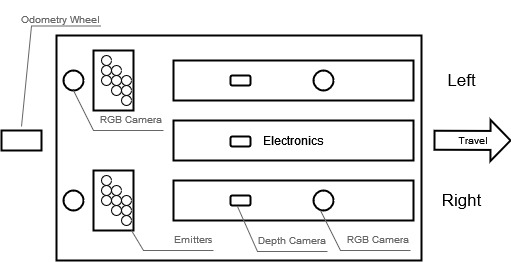
\includegraphics[width=1\linewidth]{./figures/physical-system-overhead.jpg}
		\caption{An overhead view of the system}
		\label{fig:system-overhead}
	\end{subfigure}
	\hspace{1em}%
	\begin{subfigure}[t]{.38\textwidth}
		\centering
		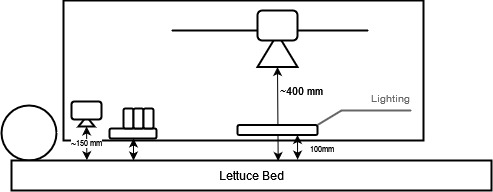
\includegraphics[width=1\linewidth]{./figures/physical-system-elevation.jpg}
		\caption{An elevation view of the system}
		\label{fig:system-elevation}
	\end{subfigure}
	\caption[Overhead and elevation views of the system]{Overhead and Elevation views of the system --- Responsibilities within the system fall into two subsystems: classification and treatment. Very roughly speaking, the classification system operates on images streamed to it from the RGB cameras, and the treatment system uses the emitters to apply chemical treatment to undesired vegetation.}
	\label{fig:system}
\end{figure}

While it is beyond the scope of this document to provide operational details of system operation, it is sufficient for this document to view the system as a targeting treatment of a two-seedline single bed with three subsystems: \textit{odometry}, \textit{classification}, and \textit{treatment}.   

\section{Physical System Characterization}
There are a few measurements that establish the relationship of system components with each other. These measurements will be used to determine the position of the treatment subsystem as the overall system moves along a planting bed.


\subsubsection{Sensor+Lens Position, Capture, and Distortion}
\label{sec:sensor}
The objective of this phase is to determine two values, the pixel to ground distance relationship and the height of the optical sensor, as well as the amount of optical distortion introduced by the lens.  The height of the sensor will vary with the depth to which the entire weeding system sinks into the bed.
\begin{figure}[H]
	\centering
	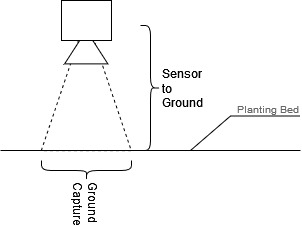
\includegraphics[width=0.25\linewidth]{./figures/sensor-calibration.jpg}
	\caption[Sensor measurements and ground capture]{The ground capture distance and sensor-to-ground measurements will vary based on the distance the entire system sinks into the planting bed. The distance to the ground can be obtained using the subset of the depth camera measurements that are unobstructed.}
	\label{fig:sensor-dimensions}
\end{figure}

No forward motion of the weeding system will be required for this stage of measurements. Measurements can be taken while the system is at rest on a hard surface, but the distance from the bed to the sensor will likely differ from measurements in the laboratory or used in calculations.  The sensor to ground distance is 431.8 mm.

The specifics of the sensor associated with classification:
\begin{enumerate}
	\item{Basler 2500-14c}
	\item{Onsemi MT9P031 sensor}
	\item{Edmund Optics 6mm Lens \#33301}
\end{enumerate}

The ground capture details of this configuration show a 41 cm x 31 cm image with 0.01 cm per pixel \footnote{Calculations provided by the Pix4D spreadsheet found here: https://support.pix4d.com/hc/en-us/articles/202560249-TOOLS-GSD-calculator}

A somewhat related procedure, but one that will be performed under laboratory conditions is the characterization of the distortion introduced by the lens in images of a checkerboard test target. 
\subsubsection{Odometry Characterization}
The odometry system is used to determine the distance traveled by the weeding system. It consists of a mechanical wheel, 920 mm in diameter, with an attached 1200 pulse per revolution encoder. Under ideal, friction-free conditions, therefore, the system will produce pulses according to this formula:
\begin{align}
\frac {wheel\ circumference}  {rotational\ pulses},\  or\  \frac {\SI{920}{\milli\meter}} {1200\ pulses} = 0.7667\ pulses\ per\ mm
\end{align}

Under field conditions, however, the odometry subsystem will not maintain this rate of pulse production, as soil conditions will lead to lower pulse counts per mm of travel. An additional complication is false pulses introduced by electrical noise and mechanical vibration.  It is, for instance, possible to induce an encoder pulse by striking (forcefully, not a gentle tap) the encoder enclosure, making it seem as if forward motion is taking place in the absence of wheel movement. These false readings affect high pulse rate encoders (the encoder in the author's office is 5000 pulses per rotation (PPR)) more than they affect the lower pulse rate encoder used in the field, so attempts will not be made to separate this effect the effect of soil conditions. False pulses introduced by electrical noise are mitigated by proper grounding and are ignored in these tests.

The number of pulses per millimeter from a standing start will use this procedure:
\begin{enumerate}
	\item{The current pulse count is recorded or reset to zero.}
	\item{The tractor tows the weeding system approximately 3 meters away and halts.}
	\item{The current pulse count is noted.}
	\item{A laser distance system will be used to establish the distance traveled.\footnote{A Leica Disto D1, with accuracy +/- 2 mm at 40 meters will be used.  Details here: https://shop.leica-geosystems.com/buy/disto/d1}}
\end{enumerate}
This test will establish pulse rate to distance mapping for those conditions. To establish an overall average pulse count it will be necessary to repeat this test for under a variety of soil conditions. While this procedure will characterize the odometry subsystem be accurate over long distances, the key distance for the overall system is  from the leading edge of the image captured to the trailing edge of the emitters.  Additionally, this is a manual process, and as such will suffer from those errors. Consequently, this procedure will be used only in early stages of the project.
Additionally this will characterize only one of the four movement scenarios that must be characterized: stop-to-stop, stop-to-in-motion, in-motion-to-in-motion, and in-motion-to-stop.  That is, does the pulse-per-mm rate change from the case where the tractor starts, moves, and then stops to the case where the tractor is in motion over the designated distance? The recording of pulse counts and notation of distance is not an activity that is well suited to an in-motion system.   

\begin{figure}[H]
	\centering
	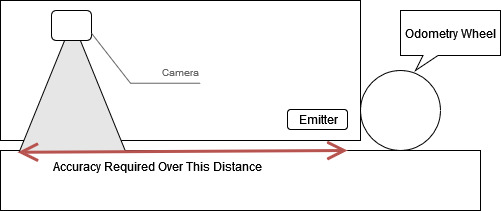
\includegraphics[width=0.75\linewidth]{./figures/system-in-field.jpg}
	\caption[Accuracy required from odometry subsystem]{The odometry subsystem requires accuracy over only a portion of a planting bed, indicated by the red line in this diagram, not the longer distances seen in other characterizations. The distance from the center of the camera to the center of the emitter in the leading edge row of the emitter plate based on an average of three measurements was 0.3479 m. While the aforementioned manual procedure can accommodate this shorter distance, it may not be the case that starting and stopping motion over this distance will lead to accurate results.}
	\label{fig:required-accuracy}
\end{figure}

To relate PPR to the distance between the camera capture and emitters, forward and rear line sensors will detect lines placed a known distance apart as the system passes overhead.
\begin{figure}[H]
	\centering
	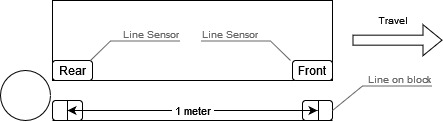
\includegraphics[width=0.75\linewidth]{./figures/determine-ppr-per-meter.jpg}
	\caption[Determine PPR per meter]{Lines are placed a known distance apart -- the 1 meter value indicated here is just for illustration and may not be indicative of the final length used -- and are detected as the system passes overhead. This technique will use Seeed Studio Line Finder part 101020172. The pulses over this distance can then be used to calculate the true PPR to ground-distance relationship under those conditions.}
	\label{fig:ppr-to-meter}
\end{figure}

This approach will be used to capture the PPR to distance relationship under all four motion conditions. In this scheme, the pulses observed between the starting and ending lines will yield the true pulse rate to distance ratio.

\subsection{Non-movement of odometry wheel}
\label{section:non-movement}
Under certain circumstances, the physical system may show forward movement (e.g., the tractor moves forward), but the odometry wheel does not turn, as mechanical issues interfere with normal rotation. In this instance, the wheel is dragged forwards, but as the system depends on wheel rotation to calculate travel distance both image acquistion and treatment will be adversely affected. In image acquisition, this will appear as gaps on acquired images, a fault that can be identified through manual inspection of images taken of a tape. Depending on the severity of the non-movement, adjacent images will show overlap inconsistent with other images or no overlap whatsoever. The latter case might show adjacent images with "53ft" and "55ft" visible in images where the ground capture distance is 6".
\begin{figure}[H]
	\centering
	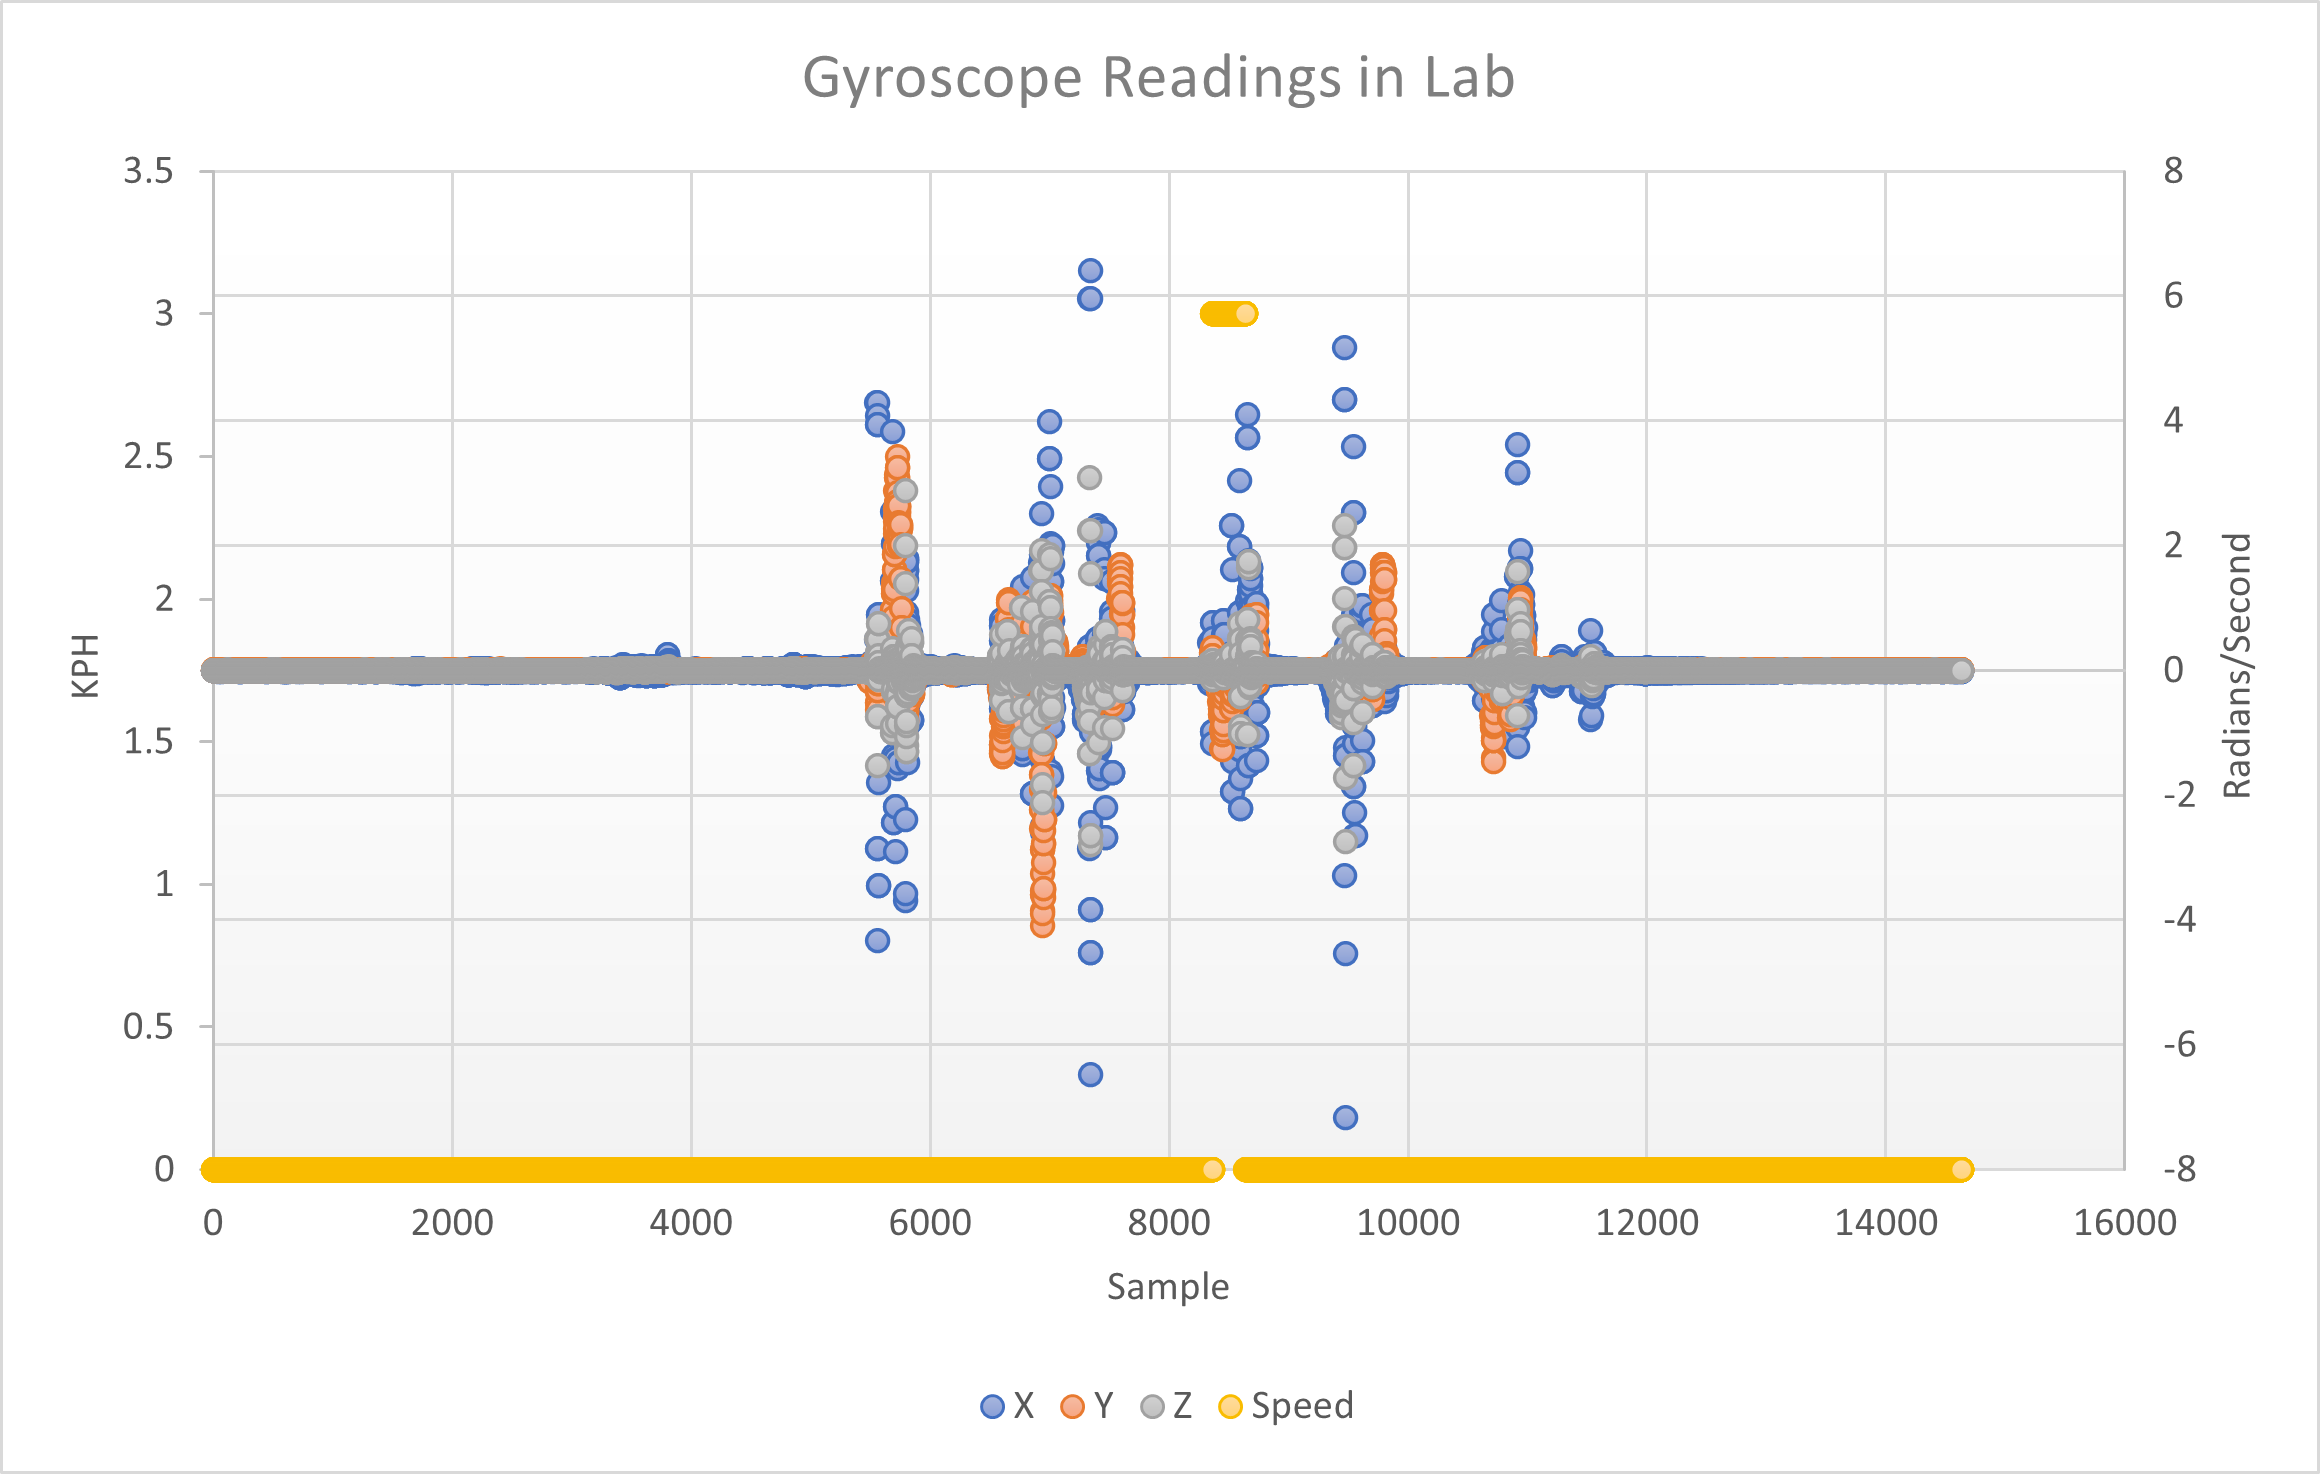
\includegraphics[width=0.75\linewidth]{./figures/imu-readings-in-lab.png}
	\caption[Detection of system movement]{This chart shows gryoscopic readings obtained in test where the camera was periodically moved back and forth along a sliding rail. The readings above and below zero indicate system movement. Readings of zero indicate that no movement was detected. The graph shows a disconnect between the gyroscopic readings and the lack of movement from the odometry wheel. There is one instance where the wheel does report motion, correlating with the gyroscopic readings.}
	\label{fig:gyro-readings}
\end{figure}
While detecting and notifying the operator of this case during operation may be desirable, as mechanical remediation can then be used, a first step is to show that this situation can be reliably detected. Figure~\ref{fig:gyro-readings} shows the relationship between movement and the gryoscopic readings and movement. In this plot, odometry readings indicate that there is no forward movement where there is movement detected. This relationship will be used to craft a real-time solution where non-movement of the wheel is noted during operation.

\subsection{Camera to Emitter Orientation}
The camera has two offsets from the leading edge of the emitter that are of concern: the distance offset along the X axis and the distance offset in the Y axis. That is, how far forward the camera is from the emitters, and how close the center of the camera is to the center of the middle emitter of the leading edge. These offsets are used to answer two questions when applying a treatment to vegetation: which emitter should be used to treat the vegetation (the Y offset) and has the weeding system moved forward enough such that that emitter is directly above the vegetation (the X offset).

\begin{figure}[H]
	\centering
	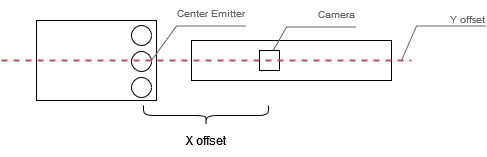
\includegraphics[width=0.75\linewidth]{./figures/camera-to-emitter-relationship.jpg}
	\caption[Determine relationship between camera and emitter]{The relationship between the camera placement and the emitters has two distances that are of of interest: the distance along the X axis between the center of the camera and the center of the emitters occupying the leading edge of the plate and the distance of the center of the camera to the left or right of the center of the middle emitter in occupying the leading row. While every attempt will be made to align the camera and emitters mechanically, they are unlikely to have their centers perfectly aligned.}
	\label{fig:camera-to-emitter-relationship}
\end{figure}

The determination of the X offset has already been discussed: 0.3479 m, based on an average of three measurements. To obtain the offset in the Y  axis, a laser will be trained on the center of the middle emitter, and the location of the laser beam captured in the image used to determine the offset.

\begin{figure}[H]
	\centering
	\begin{subfigure}[t]{.38\textwidth}
		\centering
		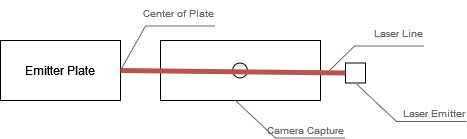
\includegraphics[width=1\linewidth]{./figures/camera-to-emitter.jpg}
		\caption{Determine camera to emitter alignment}
		\label{fig:camera-to-emitter-alignment}
	\end{subfigure}
	\hspace{1em}%
	\begin{subfigure}[t]{.38\textwidth}
		\centering
		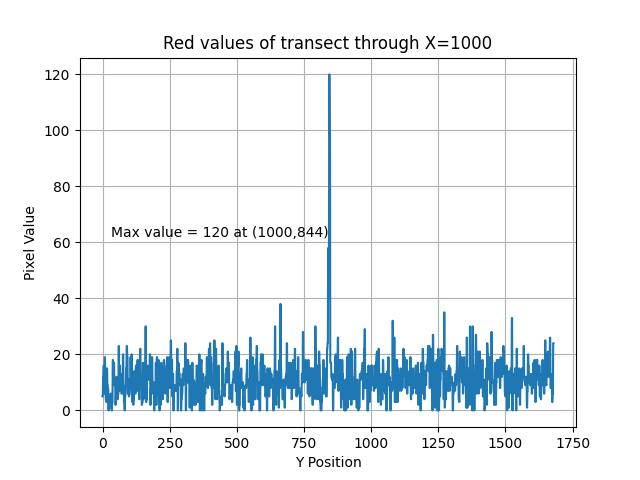
\includegraphics[width=1\linewidth]{./figures/transect-for-laser.jpeg}
		\caption{Transect through acquired image}
		\label{fig:laser-transect}
	\end{subfigure}
	\caption[Determining camera to emitter alignment]{To determine the alignment of the center of the camera to the center of the middle, leading edge emitter, a laser level is used to illuminate the center of the emitter. A transect through the image shows the beam captured in the image.}
	\label{fig:camera-to-emitter}
\end{figure}
Using the pixel width derived in Section~\ref{sec:sensor}, the center of the emitter is (0.01 * 1001) cm, or 10.01 cm from the bottom of the captured image.

\subsection{Overlap verification}
An odometry verification mode of the system software will capture and annotate images, noting every 1cm in forward motion to allow manual verification of capture accuracy.  In this verification, images of a tape measure are obtained as the weeding system is towed over it. Adjacent images should contain an overlap of 20\%\footnote{The value of 20\% is an arbitrary choice to allow for efficient stitching of adjacent images and may not be the final overlap value used. Successful stitching requires the presence of features common in both images, and as the ground is relatively featureless by itself, this figure may need to be adjusted.} The image capture strategy reflects a need to stitch consecutive images together before classification, avoiding the problem where the lack of a full view of an object prevents classification.
\begin{figure}[H]
	\centering
	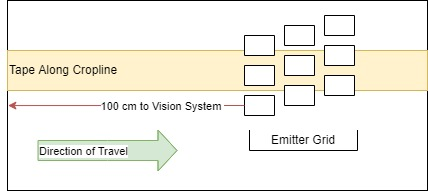
\includegraphics[width=0.75\linewidth]{./figures/test-distance.jpg}
	\caption[Test for distance measurement from emitter]{Images captured of a tape measure will be used to assess the overlap of image acquisition in  subsequent images. The accuracy of distance travel assessment will have an effect on overlap of images. It will likely be the case that the overlap will be higher than the target value of 20\% in early phases of this work, as the calculation of distance traveled will differ from the actual distance traveled.}
	\label{fig:test-distance}
\end{figure}

\subsection{Post-emitter Cameras}
The images taken from the cameras at the trailing edge of the emitters will not be stitched together, so a basic image capture will suffice. While overlap of the images is not planned or even important to the task of spray assessment, capture will not be carried out strictly according to the size of the capture area. The post-emitter camera is a Basler 1920-14gc camera equipped with a 4mm focal length lens, position 170mm from the surface. This results in a captured area of 100mm x 180mm. As previously discussed, the determination of travel distance will differ from the actual travel distance in uncalibrated systems. To allow for this error, an overlap value of 10\% will be used in captured images. As with the images captured for use in the classification system, these cameras must capture each portion of the tape.

\begin{figure}[H]
	\centering
	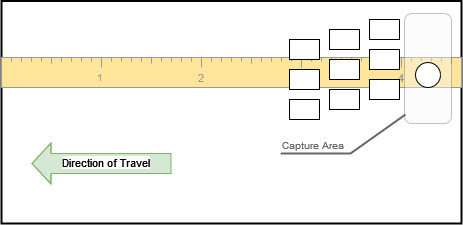
\includegraphics[width=0.75\linewidth]{./figures/test-of-distance-post-emitter.jpg}
	\caption[Test of capture for post-emitter cameras]{Images captured of a tape measure will be used to assess the capture accuracy of the post-emitter cameras.}
	\label{fig:post-emitter}
\end{figure}

\subsection{Field Tests}
Field tests will be conducted at the Yuma Agricultural Center of the University of Arizona with the integrates system in two phases: dry-run (data collection), and wet-runs. Prior to the execution of the data collection phase, however, two calibration activities will be carried out. Once executed, repeating this calibrations will not be required unless there there is a change in any physical equipment (this applies primarily to the vision and odometry subsystems).
\subsubsection{Dry-Run and Data Collection}
While each run of the system will produce usable data, these dry runs will involve only the collection of speed, timing, classification, and imagery. There is no need for a complete and integrated treatment subsystem in these tests, but this phase must be preceded by the calibration tests detailed previously.
 In these runs, the system will collect a series of crop row images, each taken with 20\% front overlap. The images collected in this phase will be used for training in future runs, so runs early in this phase are unlikely to result in acceptably accurate classification. Accuracy is expected to improve and will gate the transition to the next phase. Accuracy rates for phase exit will be 3\% false identification of crop as weeds, and 95\% correct identification of weeds as weeds.
The size of the each image set collected in this run will be dependent on several factors:
\begin{enumerate}
	\item{The size of the Region of Interest (ROI) --- the vision system proposed for this project (Basler) supports the notion of an ROI that may be a subset of the full capability of the sensor. Suppose that a strip above and below the crop line can be ignored. Capturing and processing this information may not be worthwhile.}
	\item{The compression rate of the camera system --- there is a tradeoff between image quality and the amount of compression applied. A 5 mega-pixel image contains 15 MB of data, but may be only 1 MB after compression. The image produced by the Basler acA1920-gc camera, for instance is 452 KB.}
	\item{The ground distance captured in each image}
	\item{The length of each planting bed row and the number of rows}
\end{enumerate}
Each image footprint is dependent on selections made for the vision subsystem. Using the values for a Basler acA1920-gc with a 5mm focal length lens\footnote{This camera was the only one available to the author at the time of this writing, and may not be chosen for the final project}, the image captured has these characteristics:
\begin{align}
	x = \left( \frac {elevation} {focal\ length} \right) \ *\ sensor\ width,\ or\ \left( \frac {502mm} {5mm} \right) 4.2mm = \SI{437.388}{\milli\meter} \\
	y = \left( \frac {elevation} {focal\ length} \right) \ *\ sensor\ height,\ or\ \left( \frac {502mm} {5mm} \right) 2.4mm = \SI{240.960}{\milli\meter}
\end{align}
The length of the planting bed and number of rows is variable, of course, but this proposal will assume there are four rows, each 20m in length. The total number of images is given by:
\begin{align}
	images = \frac {4 * 20m * \frac{1000mm} {1m}} {437.388mm * .8} = 228.63
\end{align}
The space needed for a single image capture set is:
\begin{align}
229\ images * \frac{\SI{452}{\kilo\byte}} {image} \approx \SI{103.5}{\mega\byte}
\end{align}

A \SI{500}{\giga\byte} SSD drive on the Jetson will provide a minimum of \SI{480}{\giga\byte} of free space, enough for several image collections. It is not anticipated that this space will be used, however, as image sets will be automatically uploaded to Amazon Web Services (AWS) and deleted from local media upon the completion of a run and successful upload to AWS.

\subsubsection{IMU}

Information required by the treatment subsystem is also collected during a dry-run.  As the system is towed down a row the position of the emitter plate (along with the rest of the system) will deviate from perfectly parallel to the ground. Figure~\ref{fig:emitter-level} illustrates the relationship of an emitter array perfectly parallel to the ground, however it will be the case that the plate will occupy a different position -- that is, the roll, pitch, and yaw of the plate will vary as the system is towed down the planting bed.


\begin{figure*}[t!]
	\centering
	\begin{subfigure}[t]{.38\textwidth}
		\centering
		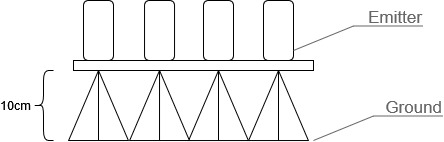
\includegraphics[width=1\linewidth]{./figures/emitter-to-ground-angle.jpg}
		\caption{Emitter to ground when level}
		\label{fig:emitter-level}
	\end{subfigure}
	\hspace{1em}%
	\begin{subfigure}[t]{.38\textwidth}
		\centering
		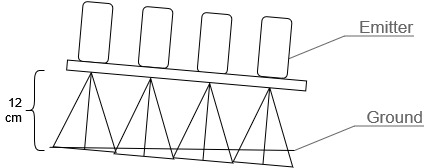
\includegraphics[width=1\linewidth]{./figures/emitter-to-ground-angle-rolled.jpg}
		\caption{Emitter to ground when rolled}
		\label{fig:emitter-rolled}
	\end{subfigure}
	\caption[Emitter plate orientation with respect to ground]{The orientation of the emitter plate will vary as the weeding system is towed down the row.  Figure~\ref{fig:emitter-rolled} illustrates the orientation when the entire assembly is rolled, as would be the case when the wheel on one side of the tractor ran over a object.}
	\label{fig:emitter-orientation}
\end{figure*}



Readings of the entire weeding assembly will be taken with each 1 mm of movement. The orientation of the two emitter assemblies are assumed to reflect the positioning of the weeder as a whole, as they are rigidly mounted. While the roll illustrated by Figure~\ref{fig:emitter-orientation} is not severe enough to require the use of a different emitter for treatment than the one that was directly overhead when the emitter plate was level with the ground, that is the intention of this data. In this case, the emitter plate may be positioned such that a treatment is possible only with an emitter adjacent to the one directly overhead. The timing of the treatment may also be affected by pitch changes (front/back up \& down).


\subsubsection{Wet-Run} 
This phase requires all subsystems to be functionally complete and integrated. During these runs, the identified weeds are treated with a tinted, non-toxic liquid.  Treatment efficacy and accuracy can be assessed in two ways:
\begin{enumerate}
	\item{Manually, by assessing the coverage of each plant by the treatment --- a manual assessment has the advantage of detailed inspection of each application, but suffers from the inevitable errors in any manual assessment. Each image is inspected by a human looking for a treatment proxy. In this case that proxy is the mark left on the ground by the application of tinted dye.}
	\item{Automatically, by capturing images of post-treatment vegetation and using those images to assess the treatment of vegetation.}
\end{enumerate}
As noted in Figure~\ref{fig:system}, the system uses cameras after the emitters to capture the state of vegetation after treatment. These images will be used to compare before (images from the classification subsystem) and after (images from the treatment subsystem) of vegetation targeted for treatment. While structural features such as shape will not be altered by a treatment, color features will be affected by the application of tinted dye. These color changes will be used as an indication of treatment efficacy.

\textit{
An unexplored option for determining treatment efficacy is using textural analysis of before and after images a specific plant. Just as the color attributes of vegetation will differ after the application of dye, so will the texture of an object. Textural analysis using Grey-Level Co-occurrence Matrix (GLCM) provides insight as to the number of times pairs of pixels with a specific relationship occur within an image. The chief problem, however is that the classification system does not generate textural data, so a textural analysis of the post-emitter image is not terribly useful. If the analysis of color changes introduced by the dye does not prove to be effective, textural analysis is the backup plan.
}

The manual assessment of spray is relatively straight-forward in that it relies on a human to determine if the spray we applied to the vegetation. This assessment does not involve the determination of the application of dye to the vegetation, but relies on a human to determine the application of the dye \textit{to the ground}.  In this scenario, a plant is considered to have been treated if it shows dye in the area directly adjacent to a leaf.
\begin{figure}[H]
	\centering
	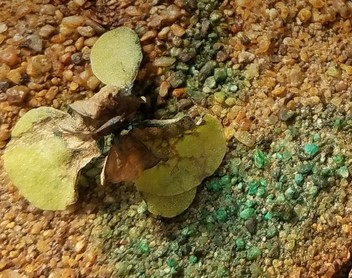
\includegraphics[width=0.45\linewidth]{./figures/dye-on-ground.jpg}
	\caption[Dye on the ground as a proxy for treatment accuracy]{The dye on the ground can be used as a proxy for treatment efficacy. This image shows dye on either side of the plant that is easily visible. As the dye on the plant is not readily visible, it will not be used to determine if this treatment was correctly applied}
	\label{fig:dye-on-ground}
\end{figure}

The automatic assessment of spray requires an image segmentation geared toward the hue of the dye, allowing the separation of treated vegetation. Once segmented, each unwanted plant is scored based on the percentage of leaf area treated. Once sufficient accuracy is achieved, treatment will transition from dyed water to dyed herbicide. Until that accuracy in achieved, weeds will be treated by manual remediation. Treatment accuracy should not be conflated with classification accuracy. While the classification of vegetation is an indication of the fate of a plant (treated or not, the intent), treatment accuracy is an indication of what actually happened. In practice, of course, the treatment accuracy must be 100\%, even if the classification is incorrect.

Manual assessment will be used in early phases as part of the development of treatment algorithms, but automatic assessment will soon follow.  Neither approach is real-time, in that the assessment is carried out after a wet-run. That is, the assessment is carried out as a process well after the treatment is applied.

\subsection{Wet-Run Without Plants}
\label{section:wet-run-without-plants}
While the intent of the system is to categorize plants, the recognition and treatment subsystems can be decoupled such that the treatment subsystem operates on a vegetation proxy, obviating the need to operate on an actual crop during development and early testing. In this case, colored dots stand in for vegetation.

\begin{figure}[H]
	\centering
	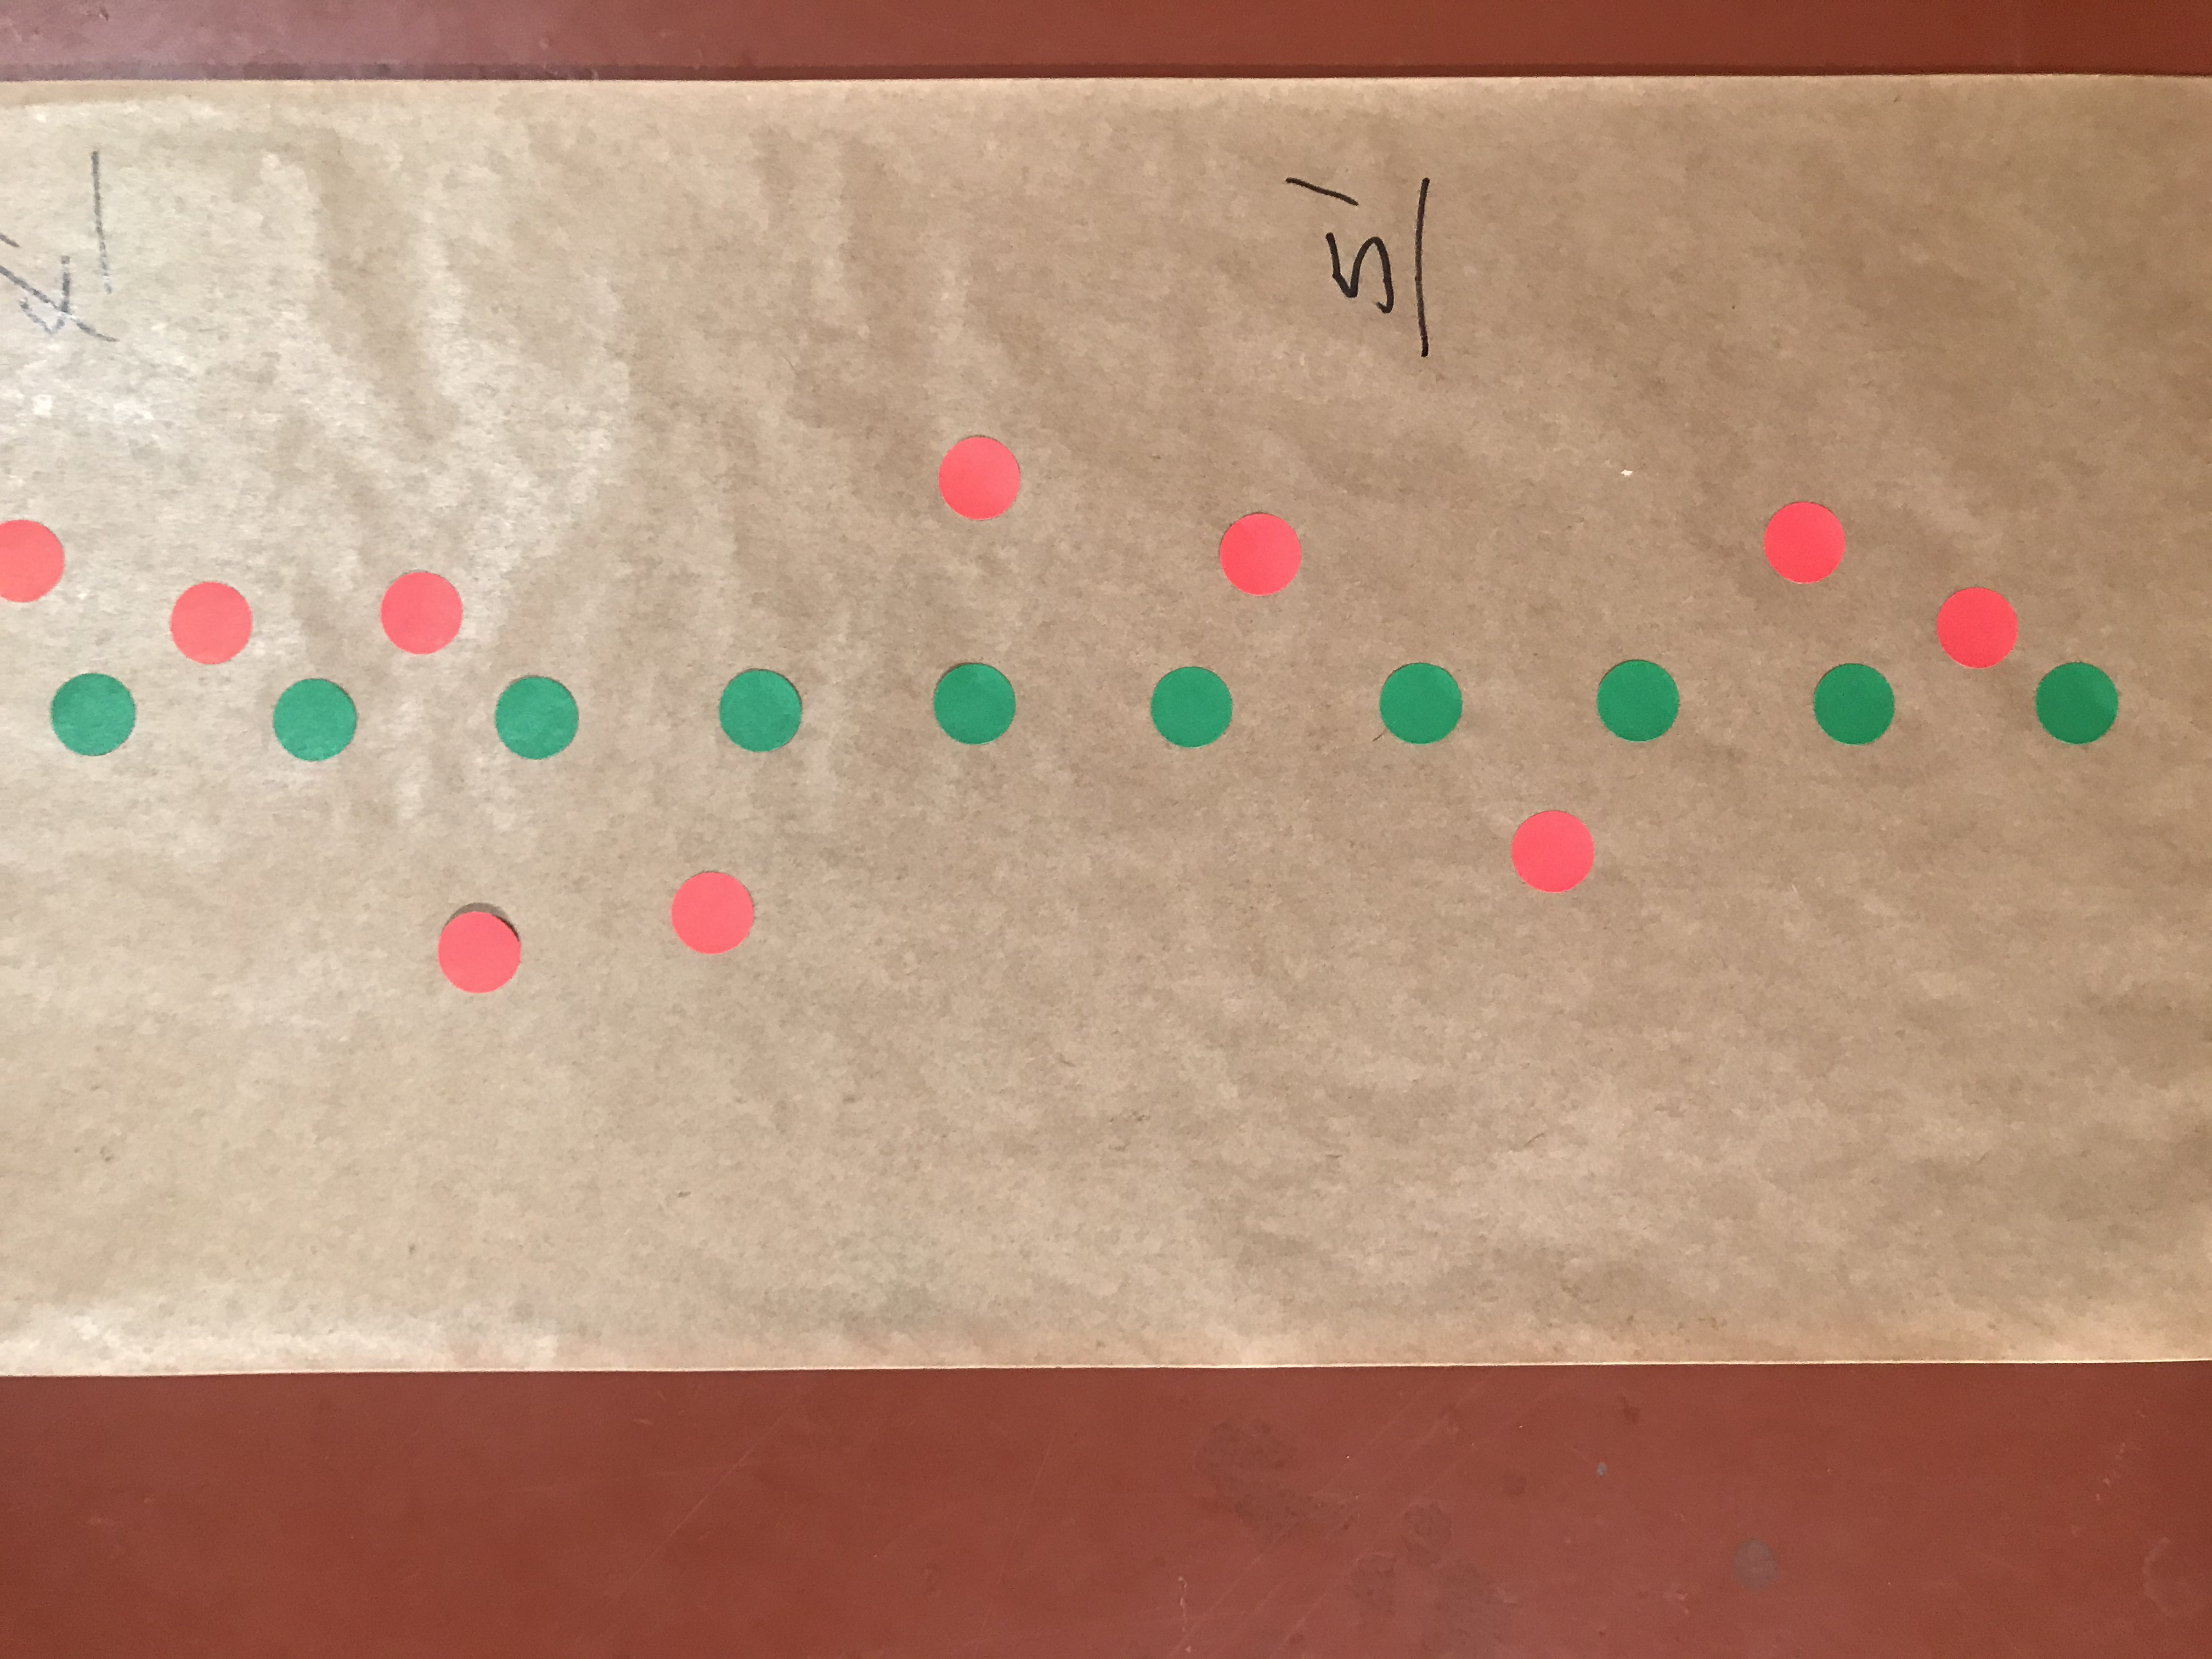
\includegraphics[width=0.45\linewidth]{./figures/green-red-dots.jpg}
	\caption[Red and green dots applied to paper for assessing spray accuracy]{The treatment subsystem can apply tinted dye to a paper target with colored dots indicating crop (green) or weeds (red). This picture is taken in the author's living room and uses a minimally absorbent paper. The concept here is that a paper target capable of absorbing dyed fluid would be used in the field.}
	\label{fig:green-red-dots}
\end{figure}
 In this case, the dots are classified with 100\% accuracy, shifting the focus to the accuracy of the treatment applied to them. Under this scheme, a short (2 or 3 meters -- the length has no impact on this scheme) segment of paper is prepared with green and red dots and affixed to the ground. The weeding apparatus is towed over the paper strip, applying treatments (within constraints of proximity to crop) to the dots classified as weeds. \footnote{There are some mechanical issues to executing on this proposal, as absorbent paper can be obtained, but the colored dots shown in the picture have a slick surface that will resist absorption of the dye. The main substrate can be something like ULINE Bogus paper, as this scheme will not require individual spray targets. Using any product that is dye-resistant will result in a bit of a mess that is not yet fully worked out.}

\subsection{Weed Populations in Different Seasons}
The tests will be conducted only over the lettuce growing season, September to March. That is, the lettuce crop will be present beside different populations of weeds over the development cycle.
\begin{figure}[H]
	\centering
	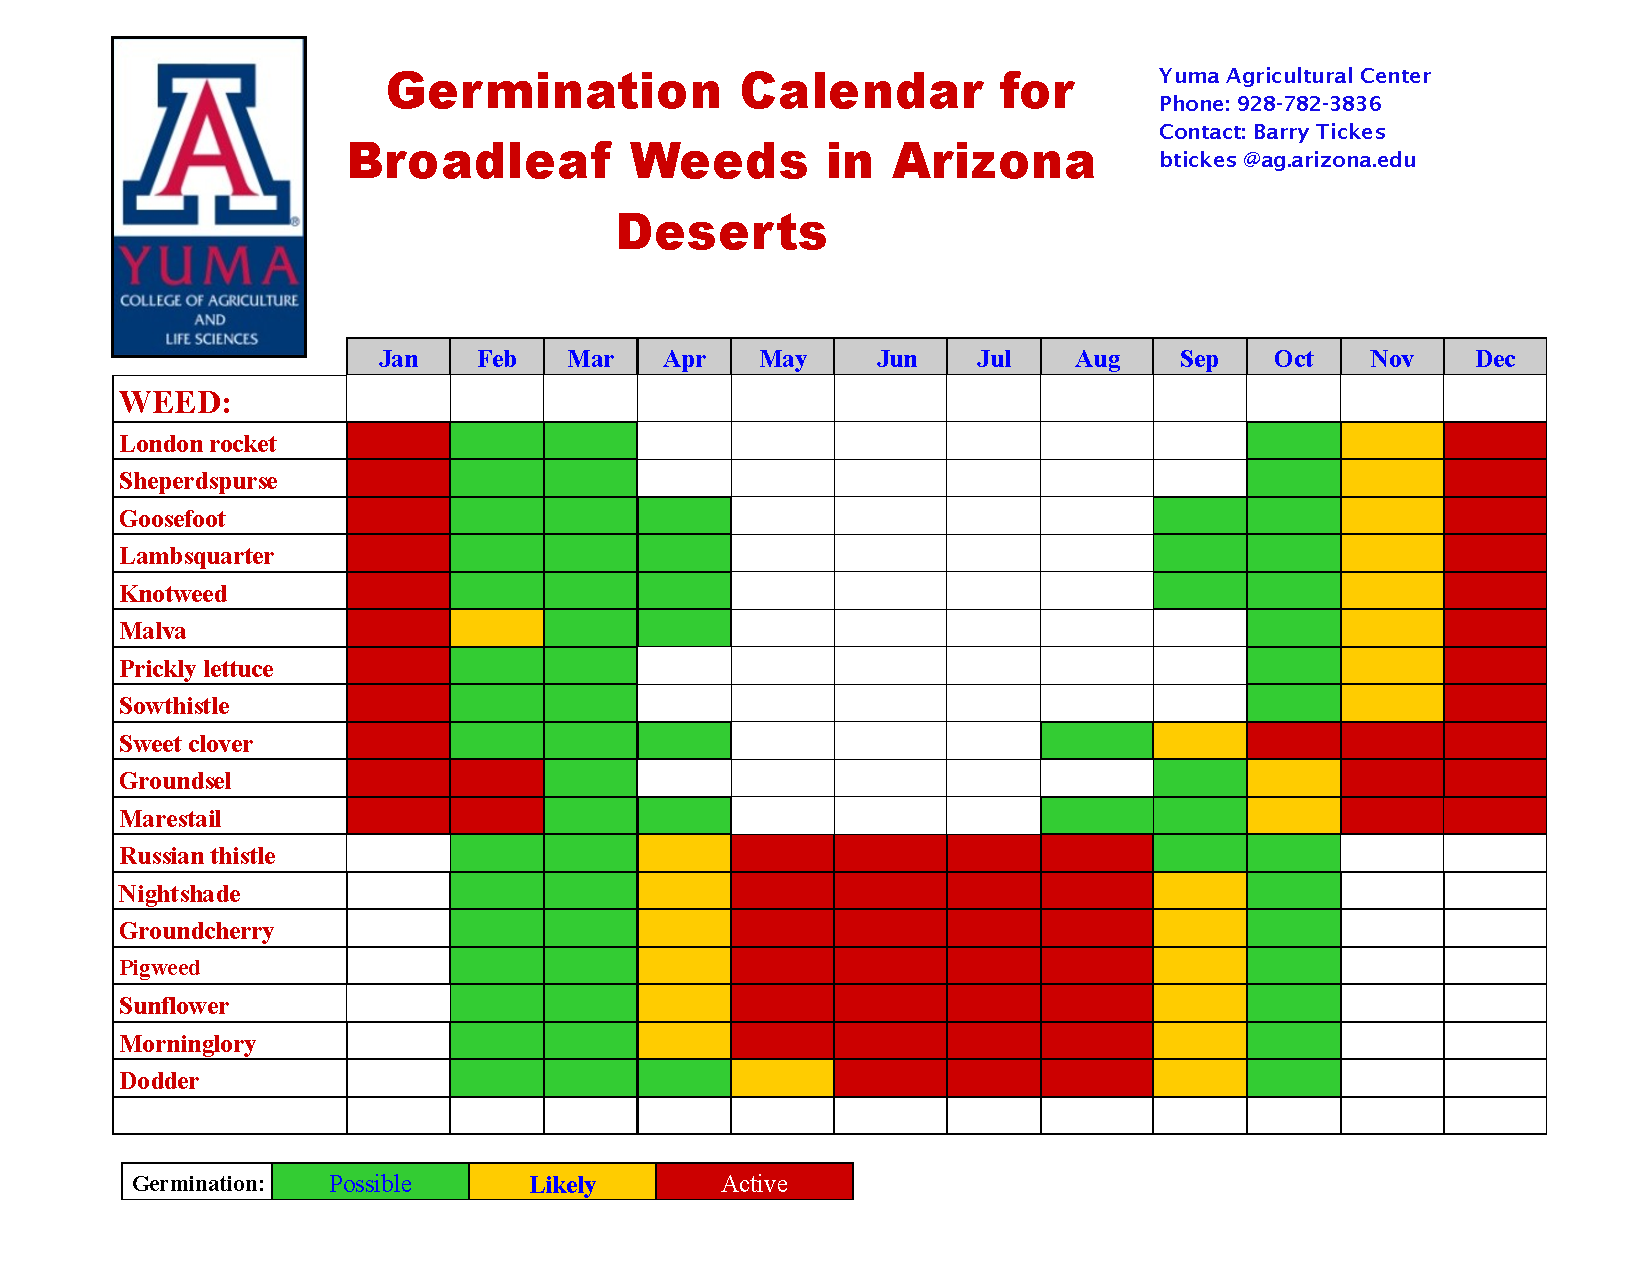
\includegraphics[width=0.75\linewidth]{./figures/broadleaf-calendar.pdf}
	\caption[Germination schedule for broadleaf weeds]{While the system will be used only within the lettuce growing season, all of the weeds listed here are listed as \textit{likely} or \textit{active} with the exception of \textit{Russian Thistle} during that time.}
	\label{fig:weed-germination}
\end{figure}



\subsection{Weed/Crop Discrimination over the Growth Cycle}
There are four factors used to classify vegetation in a previous analysis:
\begin{enumerate}
	\item{YIQ In-Phase Mean -- a color attribute of the vegetation}
	\item{Shape Index -- a shape attribute}
	\item{Length/Width Ratio -- a shape attribute}
	\item{Distance from cropline -- a positional attribute}
\end{enumerate}

While there are many other attributes extracted, these are the ones found to be most significant. Roughly speaking, however, all attributes fall into one of three categories: color, shape, or position. Position, the position of the vegetation relative to the crop line, is the sole factor that will be invariant across development cycles: if vegetation is not close to the cropline, it is likely to be a weed. As for shape attributes, as the leaves of broadleaf weeds expand across the development cycle, it is anticipated that the shape computations will remain significant due to their relative consistency. The shape attributes computed are not affected by size.
This leaves color attributes as the sole set of factors to be used at various points.\footnote{This is also one of the reasons why the images are captured using a color camera instead of a monochrome. The other reason is that the image segmentation approaches applied as part of the image processing flow are color-based.}
 The attribute identified as significant in the previous analysis in the YIQ color space encodes the orange-blue information.\footnote{The I in YIQ is orange-blue. The Q value encodes purple-green} Changes where vegetation is perceived as more \textit{green} over the development cycle are not significant in classification.

\subsection{Balanced Learning and Weed Load}


 \newpage






%REFERENCES
%Use the Vancouver Style of referencing. This is found at this website:
%http://www.ncbi.nlm.nih.gov/books/bv.fcgi?rid=citmed.TOC&depth=2 or a less detailed website:
%http://www.nlm.nih.gov/bsd/uniform_requirements.html
%
%References should be numbered consecutively in the order in which they are first mentioned in the text. Identify references in text, tables, and legends by Arabic numerals in parentheses. The titles of journals should be abbreviated according to the style used in Index Medicus. Consult the list of Journals Indexed for MEDLINE, published annually as a separate publication by the National Library of Medicine. The list can also be obtained through the Library's web site..



 


% 
% E N D  T E M P L A T E  F R O M  W O R D
%

\newpage
{
\setstretch{1.0}
\section{References}
\printbibliography[heading=none]
}

\end{document}

